\subsubsection{Réduction du domaine de NvPD par borne de distance}\label{sec:nvpd-adaptatif}

Les colonnes indépendantes de NvPD~\cite{sadiq} permettent de vectoriser une ligne. La version dense évalue encore toutes ses colonnes, même pour deux chaînes presque identiques. Notre variante reprend le principe d'un seuil croissant~\cite{ukkonen}. Elle conserve l'index de dernière occurrence de NvPD entre les essais. Elle calcule le score global avec des coûts unitaires.

Après retrait des extrémités identiques, on oriente les chaînes pour avoir \(m\leq n\). On note \(\Delta=n-m\) et \(e=j-i\). Pour atteindre la cellule \((i,j)\), il faut au moins \(|e|\) insertions ou délétions, puis au moins \(|\Delta-e|\) pour atteindre la cellule finale. Un budget de \(k\geq\Delta\) impose donc
\[
 |e|+|\Delta-e|\leq k,\qquad
 -h\leq e\leq\Delta+h,\qquad
 h=\left\lfloor\frac{k-\Delta}{2}\right\rfloor .
\]
Dans une ligne, on évalue les colonnes de cet intervalle avec la récurrence de NvPD. Lorsque le dernier match en colonne \(t\) existe, le terme correspondant vaut \(D_{i-1,t-1}+j-t\). Un prédécesseur absent de la bande reçoit la sentinelle \(k+1\), qui sature aussi chaque résultat. La borne inférieure initiale est la somme, sur les symboles, des déficits de la première chaîne par rapport à la seconde. Un chemin qui substitue les désaccords positionnels puis insère le reste donne la borne supérieure. Si ces bornes diffèrent, le premier budget vaut au moins un. Après un échec, l’algorithme~\ref{alg:nvpd-adaptatif} double le budget dans la limite de la borne supérieure.

Pour vérifier le certificat, considérons un chemin optimal de coût au plus \(k\). Tout préfixe optimal jusqu'à l'une de ses cellules peut être suivi du suffixe de ce chemin sans dépasser le budget. Le saut vers le dernier match se développe en un match et des insertions. Son prédécesseur et chacune des cellules traversées satisfont donc l'inégalité du corridor. Une induction sur les lignes donne la valeur exacte pour tous les préfixes nécessaires. Dans l'autre sens, un résultat terminal au plus égal à \(k\) provient de transitions réelles, car une sentinelle ne peut engendrer cette valeur. Une ligne dont le minimum dépasse \(k\) termine l'essai. Pour une distance \(d\) et \(s\) symboles distincts du côté des lignes, le travail sur les chaînes résiduelles est \(O(sn+m(d+1))\), par sommation des budgets successifs. Le retrait des extrémités coûte au plus un balayage linéaire des chaînes initiales. Les deux lignes occupent \(O(d+1)\) entiers et l'index \(O(sn)\).

\begin{algorithm}[htbp]
\caption{Score NvPD par budgets certifiés}\label{alg:nvpd-adaptatif}
\begin{algorithmic}[1]
\Require Nonempty trimmed strings \(A,B\), \(m\leq n\), lower and upper bounds \(L,V\)
\If{\(L=V\)} \State \Return \(L\) \EndIf
\State \(K\gets\max(1,L)\), \(T\gets\Call{LastOccurrences}{A,B}\)
\Loop
  \State \(h\gets\lfloor(K-\Delta)/2\rfloor\)
  \State Evaluate NvPD on \(-h\le j-i\le\Delta+h\) using \(T\) and two rows
  \If{the final value is at most \(K\)} \State \Return the final value \EndIf
  \State \(K\gets\min(2K,V)\)
\EndLoop
\end{algorithmic}
\end{algorithm}

\begin{figure}[htbp]\centering
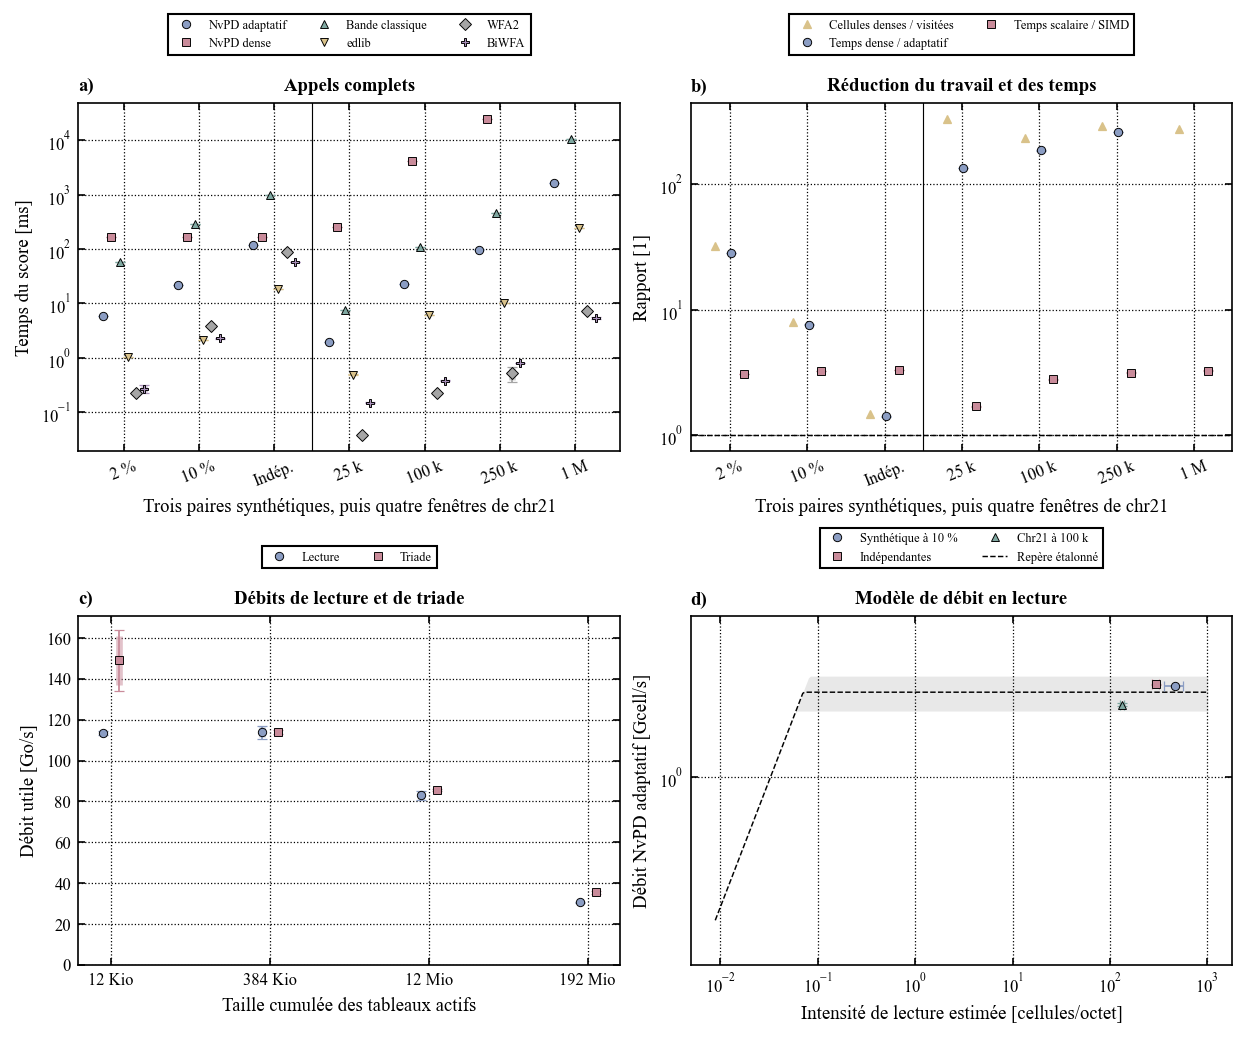
\includegraphics[width=.99\linewidth,height=.57\textheight,keepaspectratio]{../figures/cpu/nvpd_adaptatif.png}
\caption{Sur un cœur EPYC, chaque durée moyenne (a) est suivie de l'écart-type et de la demi-largeur de l'IC à 95\,\% pour cinq processus. La mention « n.m. » signale une combinaison absente. Les rapports en b) suivent les mêmes lignes. Les débits étalonnés en c) fixent le modèle de lecture en d), dont la zone grise représente un écart-type sur les paramètres.}\label{fig:nvpd-adaptatif}\sourcefig{bench/cpu/adaptive/measure.py}
\end{figure}

Le banc de la figure~\ref{fig:nvpd-adaptatif} conserve les coûts unitaires et utilise edlib comme contrôle indépendant. Deux paires synthétiques ont des taux de modification demandés de 2 et 10\,\%. Une troisième paire de 20\,000 bases contient deux chaînes tirées indépendamment. Les quatre fenêtres du chromosome 21 débutent aux coordonnées GRCh38 34\,500\,000 et CHM13 32\,882\,567. Leur distance va de 34 à 2\,336 opérations. Chaque mesure chronomètre un appel entier après une chauffe, sur le même cœur et dans un ordre tiré par bloc. Le comptage des cellules inclut les tentatives dont le budget s'est révélé insuffisant.

À 250\,000 bases, NvPD dense prend \(25{,}116\pm0{,}016\)\,s et la variante en bande \(97{,}65\pm0{,}21\)\,ms. Le rapport apparié moyen des temps atteint 257,20 (IC à 95\,\% de 256,58 à 257,82). Seules 307 bases ont été retirées aux extrémités de chaque chaîne. Les essais successifs visitent 216 millions de cellules sur une grille de 62,5 milliards. Sur les deux chaînes indépendantes, la distance atteint 10\,373 pour 20\,000 bases et le rapport des temps retombe à 1,421 (IC de 1,405 à 1,436).

Le contrôle scalaire conserve les mêmes bandes et les mêmes cellules. À 10\,\% de modifications synthétiques, les minima imbriqués permettent à GCC de traiter huit indices de match par instruction \texttt{vpgatherdd}. Le nombre d'instructions retirées par cellule passe de 25,07 à 2,74. Le temps passe de \(70{,}30\pm0{,}05\) à \(21{,}71\pm0{,}07\)\,ms. Sur la fenêtre humaine d'un million de bases, la variante en bande prend \(1{,}608\pm0{,}003\)\,s. La bande classique prend 10,485\,s, edlib 243\,ms, WFA2 7,07\,ms et BiWFA 5,41\,ms pour le même score de 2\,336. Le temps dense à cette longueur n'a pas été mesuré.

Le panneau d) adapte le modèle Roofline~\cite{roofline} aux mises à jour entières. Pour \(U\) cellules effectivement évaluées et \(Q\) octets lus estimés hors cache, le repère de débit vaut \(\min(P_{\rm L1}, B_{\rm lecture} U/Q)\). Le premier terme est le débit de la boucle NvPD en bande sur 12\,Kio, le second repose sur une lecture contiguë de 192\,Mio, au-delà du L3 de 32\,Mio du groupe de cœurs. L'expression d'une cellule demande quatre lectures d'entiers et une écriture. Les adresses se recouvrent entre cellules. Le trafic lu estimé \(Q\) compte 64 octets par remplissage L1 classé DRAM ou E/S mappée en mémoire et par prélecture manquant le L2 et le L3, à partir des événements AMD \texttt{0x4844} et \texttt{0xff72}. Les écritures et l'activité des autres cœurs échappent à cet estimateur.

Sur 192\,Mio, la lecture linéaire atteint \(30{,}64\pm0{,}21\)\,Go/s et la triade \(35{,}46\pm0{,}46\)\,Go/s utiles (moyenne et écart-type). L'estimateur des deux événements retrouve \(95{,}85\pm0{,}66\)\,\% des octets connus de la lecture. Le noyau de ligne en L1 produit \(2{,}17\pm0{,}34\) milliards de mises à jour par seconde. Les trois appels réels profilés visitent de 133 à 461 cellules par octet lu estimé et atteignent de 1,94 à 2,33 milliards de cellules par seconde. Les deux taux les plus élevés dépassent légèrement la moyenne de l'étalon L1 et restent dans sa dispersion. Le modèle situe ces appels du côté du noyau de calcul. Les accès en cache et les instructions sont regroupés dans le terme \(P_{\rm L1}\).

\synthese{À un million de bases, les quatre essais de NvPD en bande calculent 3,69 milliards de cellules, soit 0,37\,\% de la grille. À 250\,000 bases, le gain temporel mesuré atteint 257,2 sur le NvPD dense d'un cœur EPYC.}
